\chapter{Análisis de requisitos}
\label{chap:requisitos}
\section{Funcionalidades}
Esta aplicación dispoñerá de catro funcionalidades principais:
\begin{itemize}

    \item \textbf{Menú principal}: Funcionalidade "de enlace" co resto das funcionalidades. É a base da aplicación.
    
    \item \textbf{Dicionario}: Apoiarase nunha base de datos deseñada con \textit{Room} para gardar as palabras e poder seleccionar unha aleatoriamente á hora de comezar unha partida. Poderanse eliminar e engadir palabras. Non se permitirá utilizar o dicionario baleiro no resto de funcionalidades. Non se poderá introducir unha palabra maior a 17 caracteres por cuestión de espazo. Haberá comprobación dos caracteres introducidos.
    
    \item \textbf{Modo un xogador}: Esta funcionalidade consistirá en permitir ao usuario poder xogar de maneira individual. Neste caso, a aplicación escollerá unha palabra aleatoria dende un dicionario (podendo ser este ampliable polos usuarios) situado nos propios arquivos da aplicación e presentaralla ao usuario por pantalla para que trate de adiviñala. Ademais a aplicación amosará un teclado 'artificial' sen necesidade de usar un do sistema. Ao seleccionar unha letra dese teclado amosarase sombreada e non será posible volver a seleccionala.
    
    
    \item \textbf{Modo multixogador}: Nesta funcionalidade permitirase a dous usuarios xogar un contra outro. O funcionamento segue o mesmo modo que o dun xogador (hereda a súa vista) pero cun contador no que se amosa o tempo restante para elexir unha letra. Se este tempo expira, o xogador será eliminado. Gañará o xogador que adiviñe antes a palabra para evitar situacións de empate ou o que quede sen ser eliminado. Esta funcionalidade encárgase da parte de autencicación de usuarios e comunicacións en liña. Será necesario engadir todo o proceso de autentificación e unha sala de espera virtual para iniciar a partida cando os dous xogadores se presenten como listos.  \cite{mail-login} \cite{awesome-validation} \cite{mail-login2} \cite{firebase-loggin}
    
\end{itemize}
\begin{center}
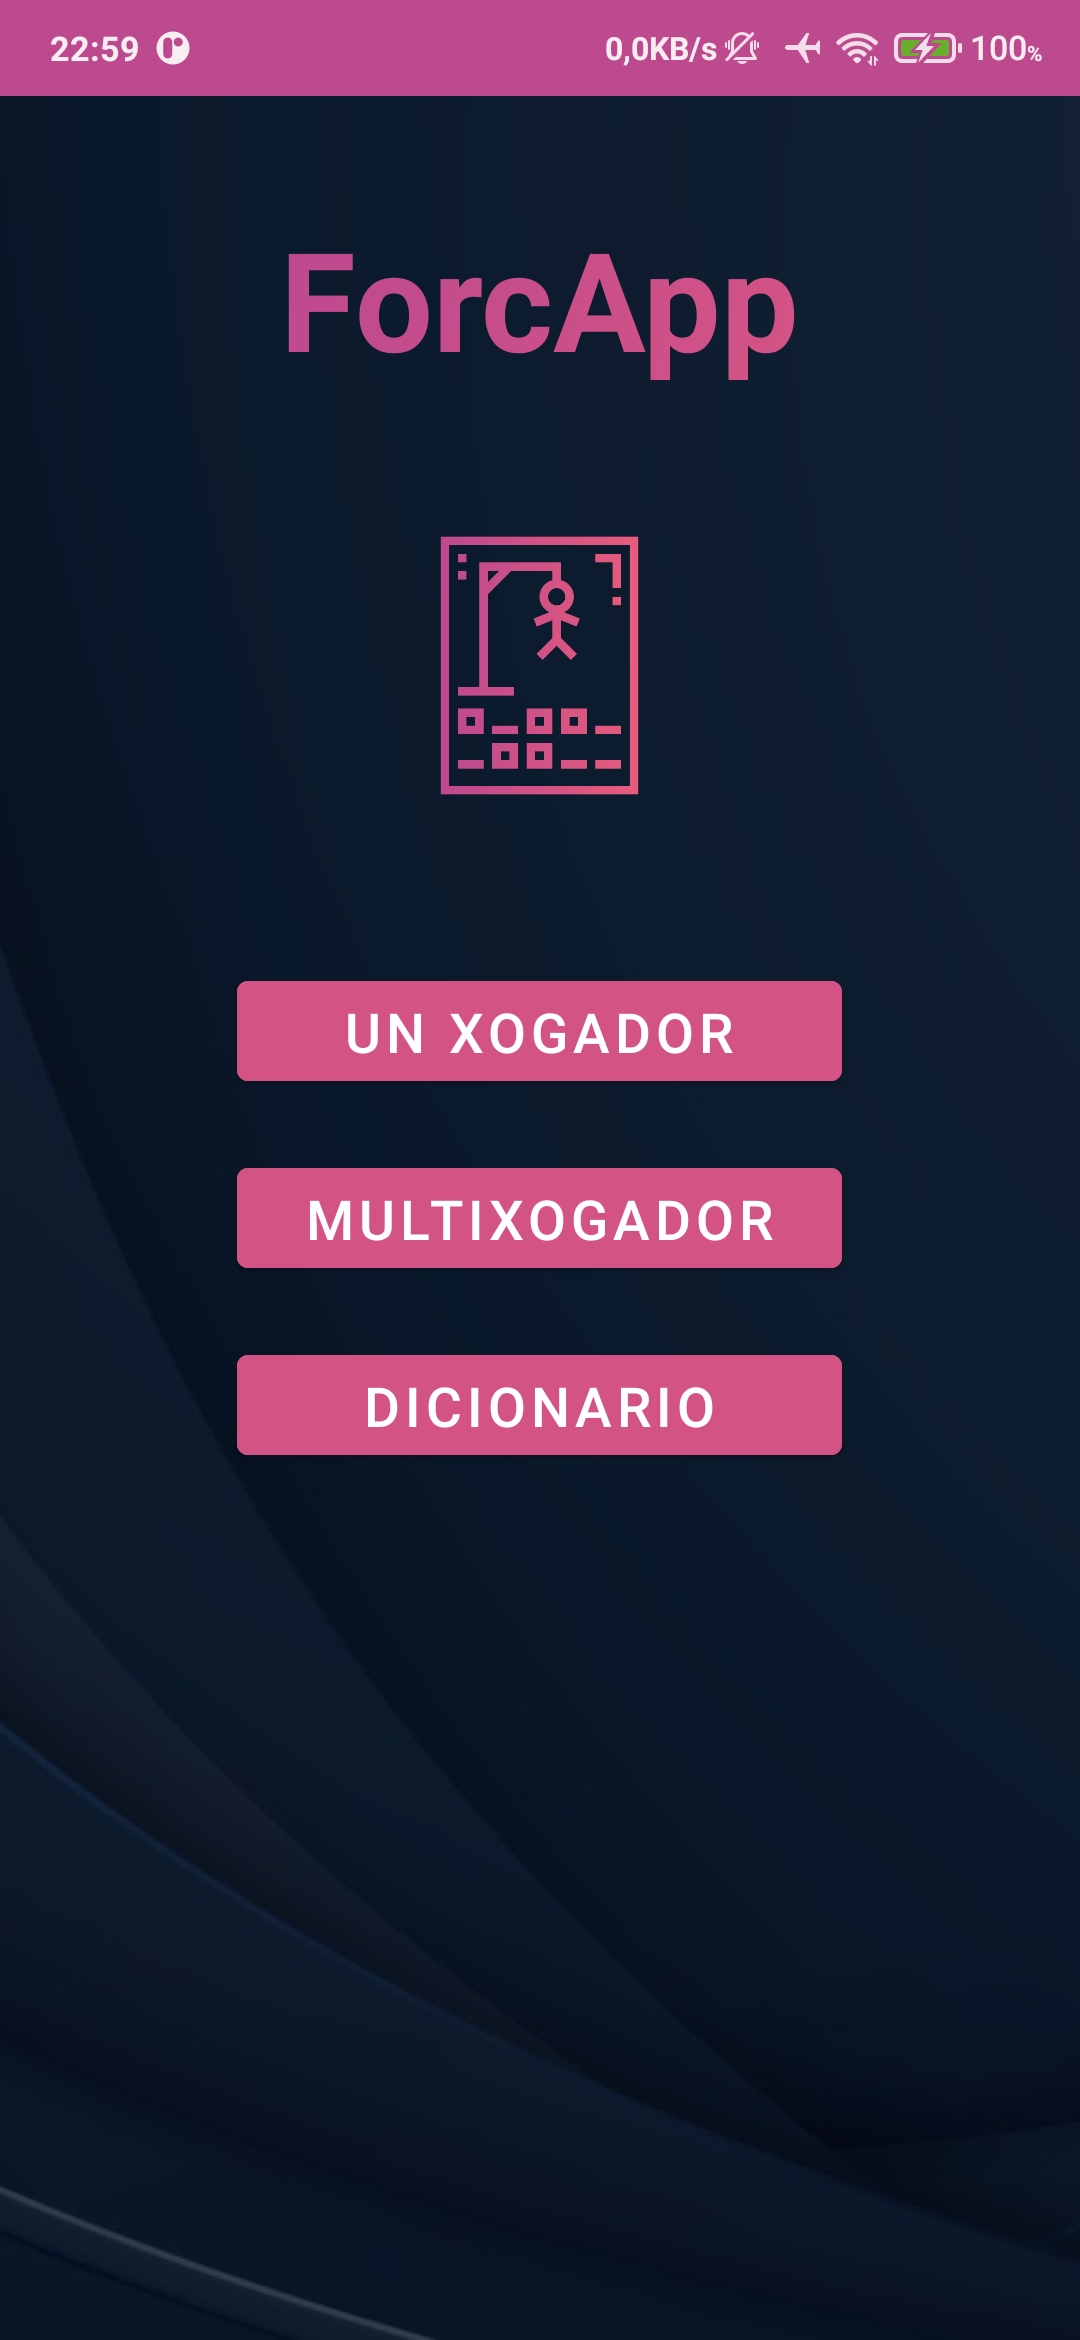
\includegraphics[scale=0.105]{imaxes/menu.jpg}
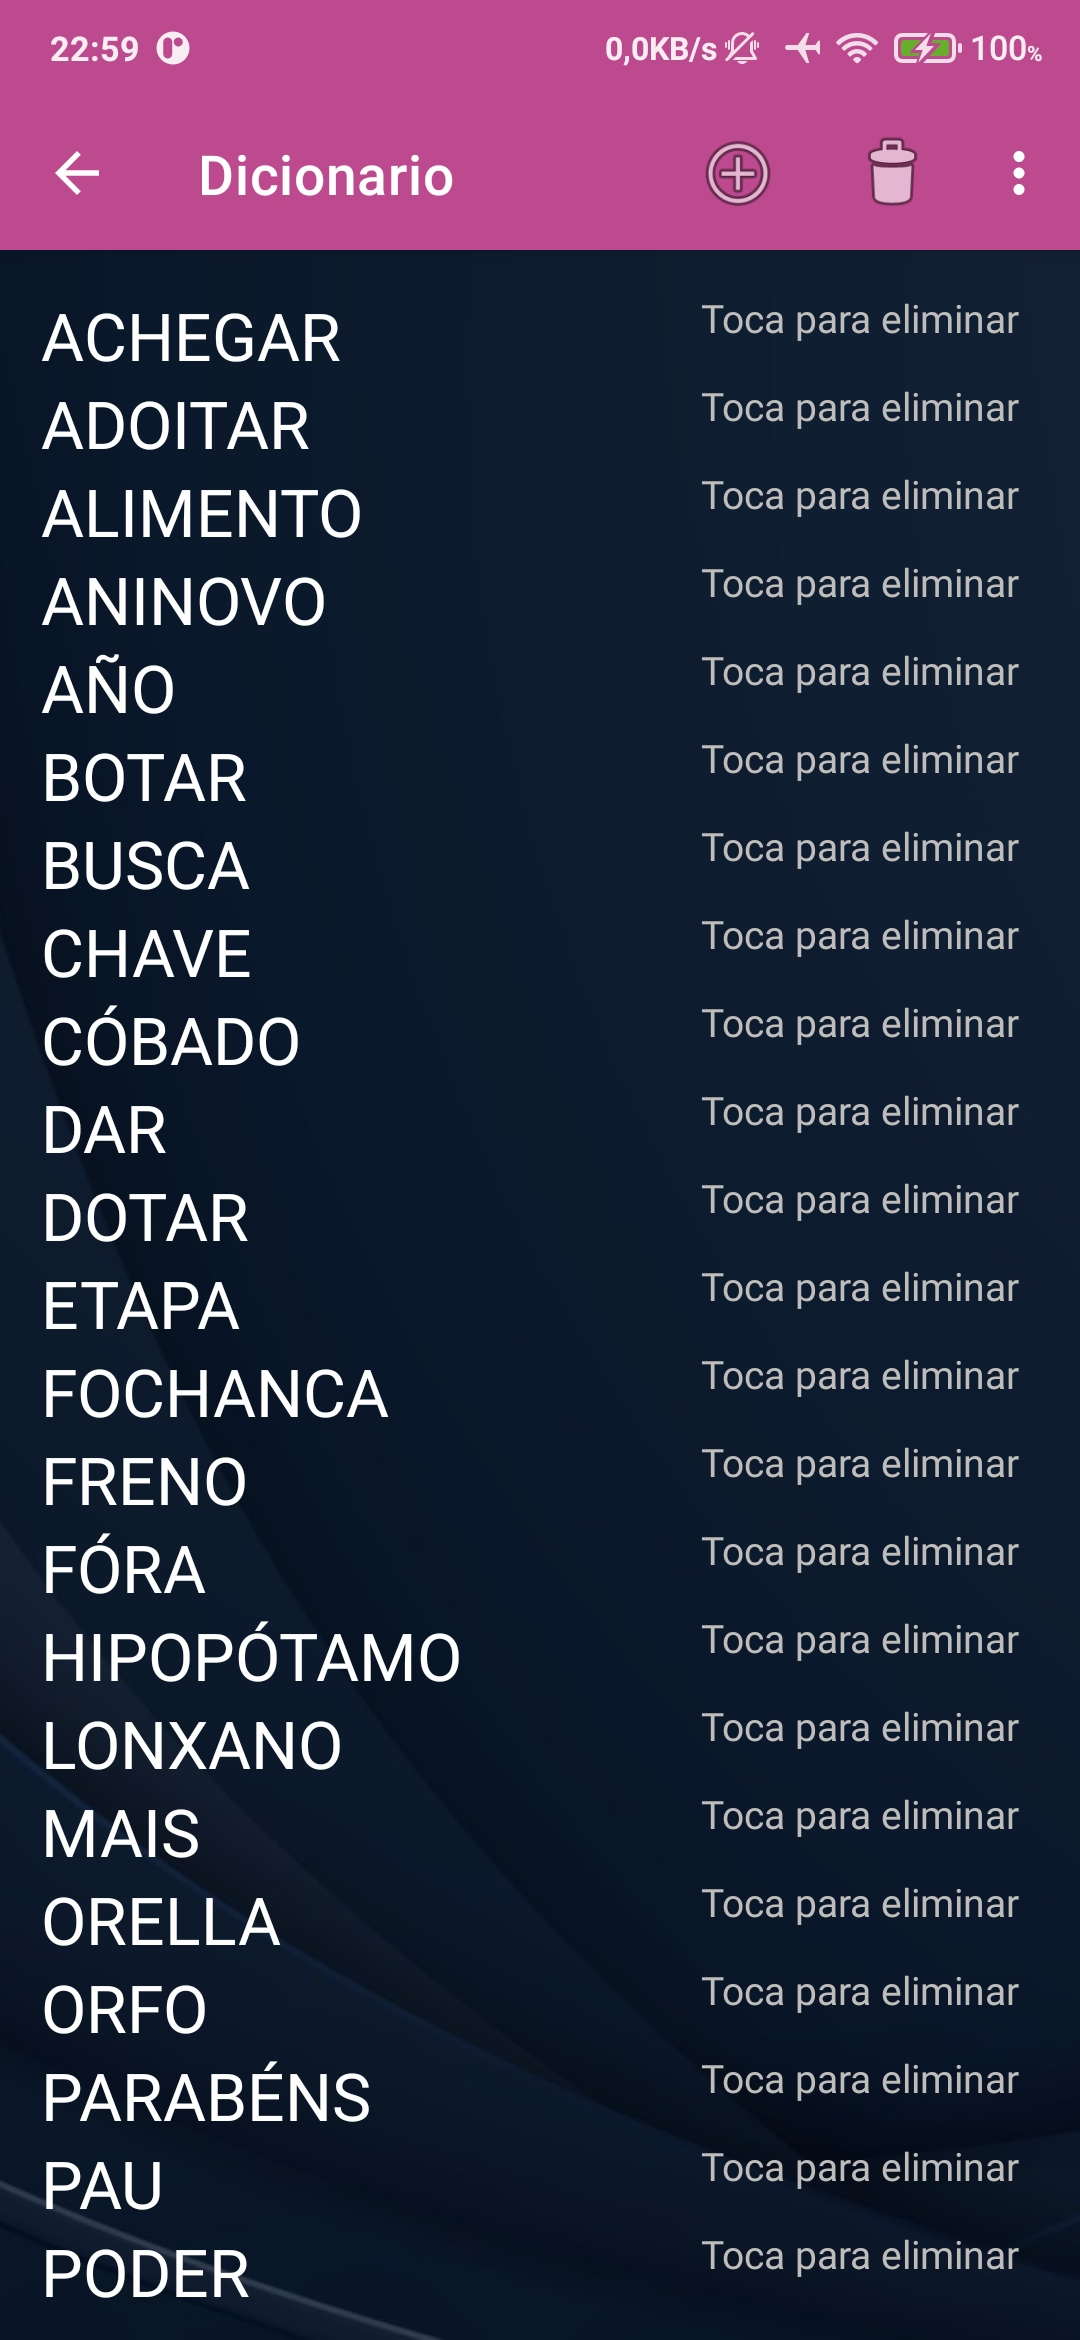
\includegraphics[scale=0.105]{imaxes/dicionario.jpg}
\end{center}
\begin{center}
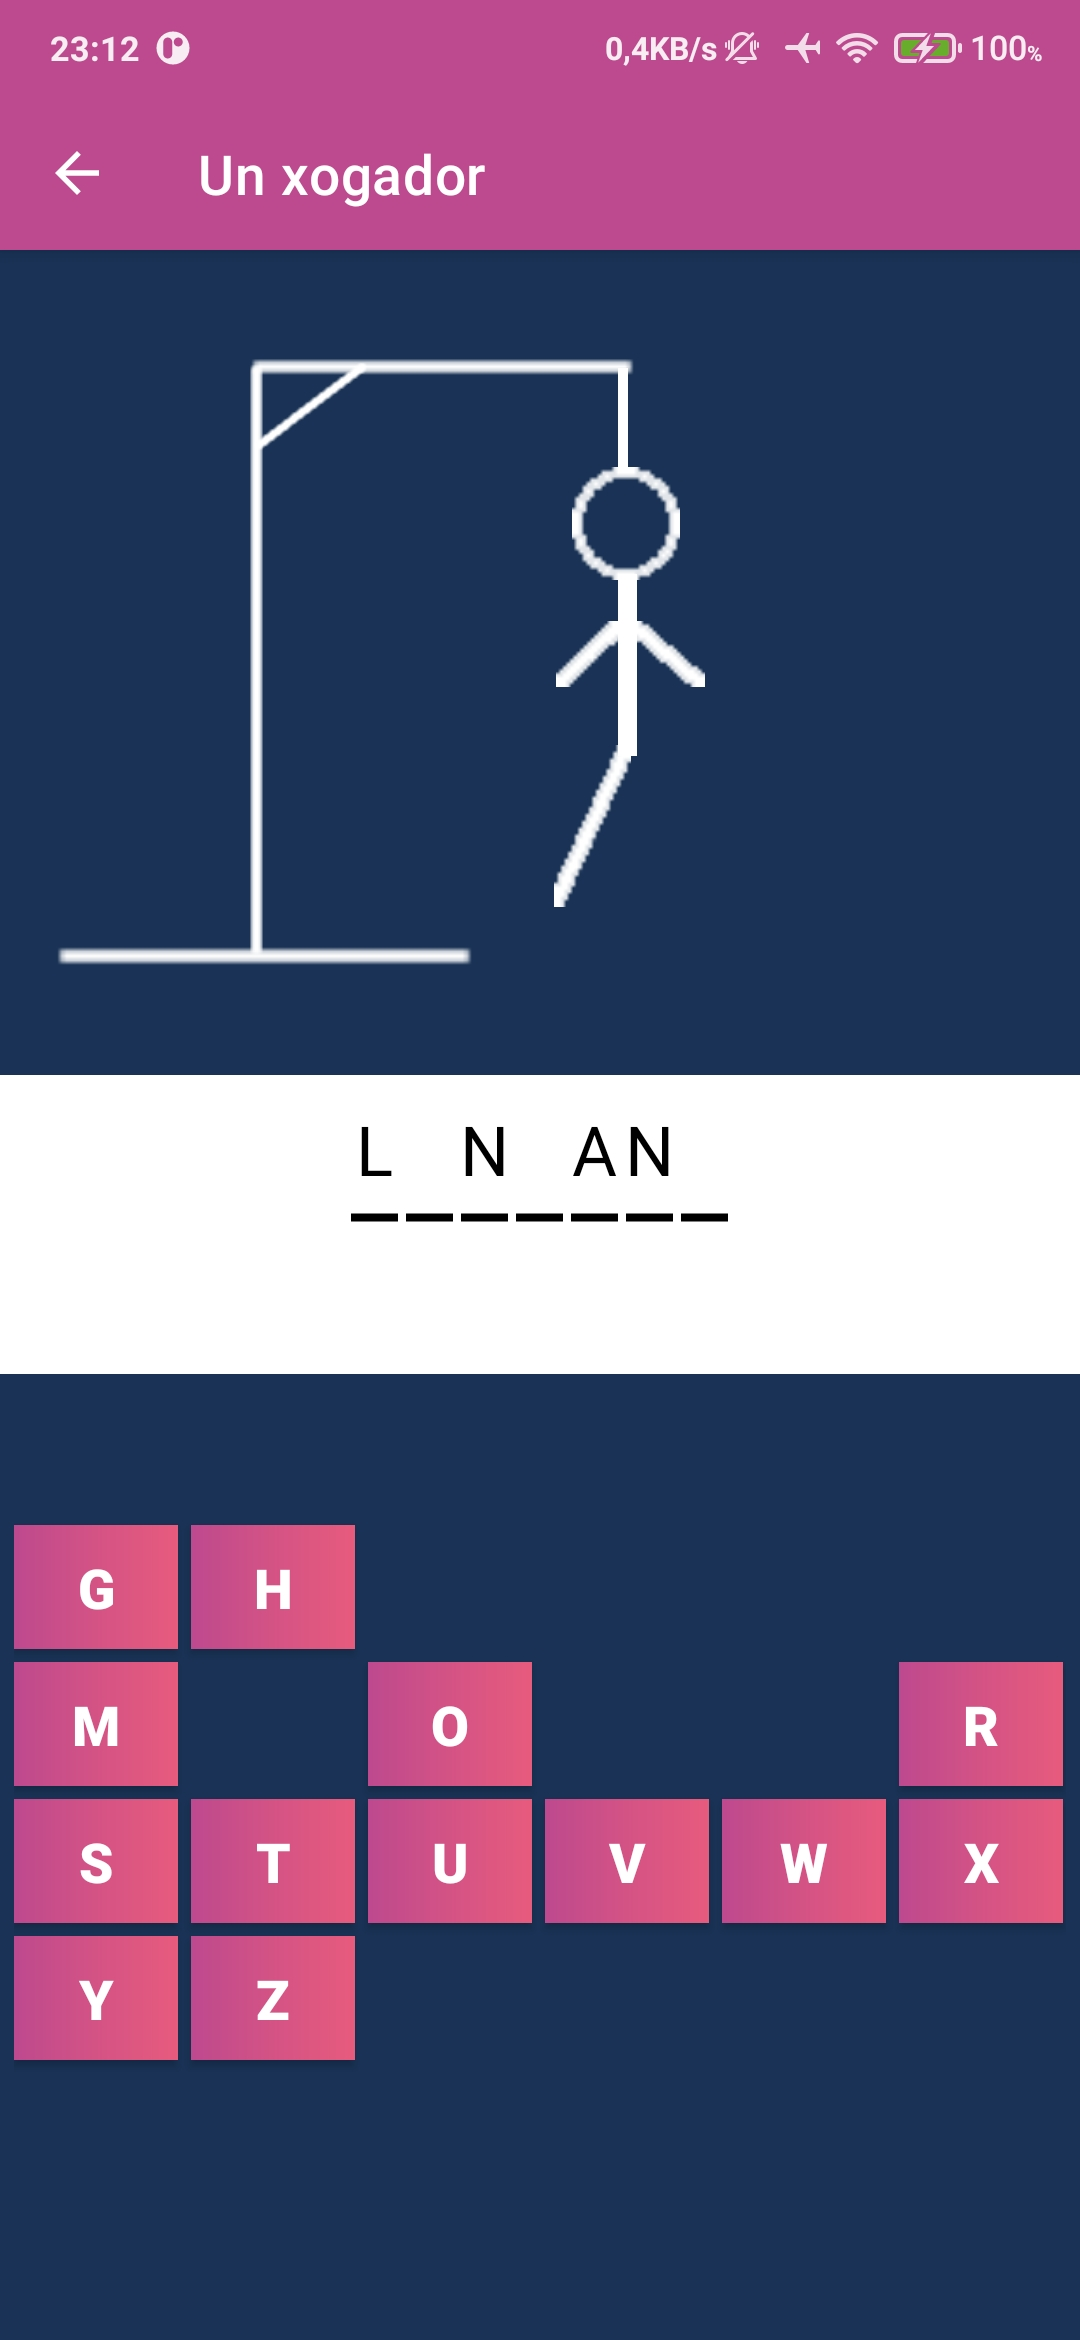
\includegraphics[scale=0.105]{imaxes/singleplayer.jpg}
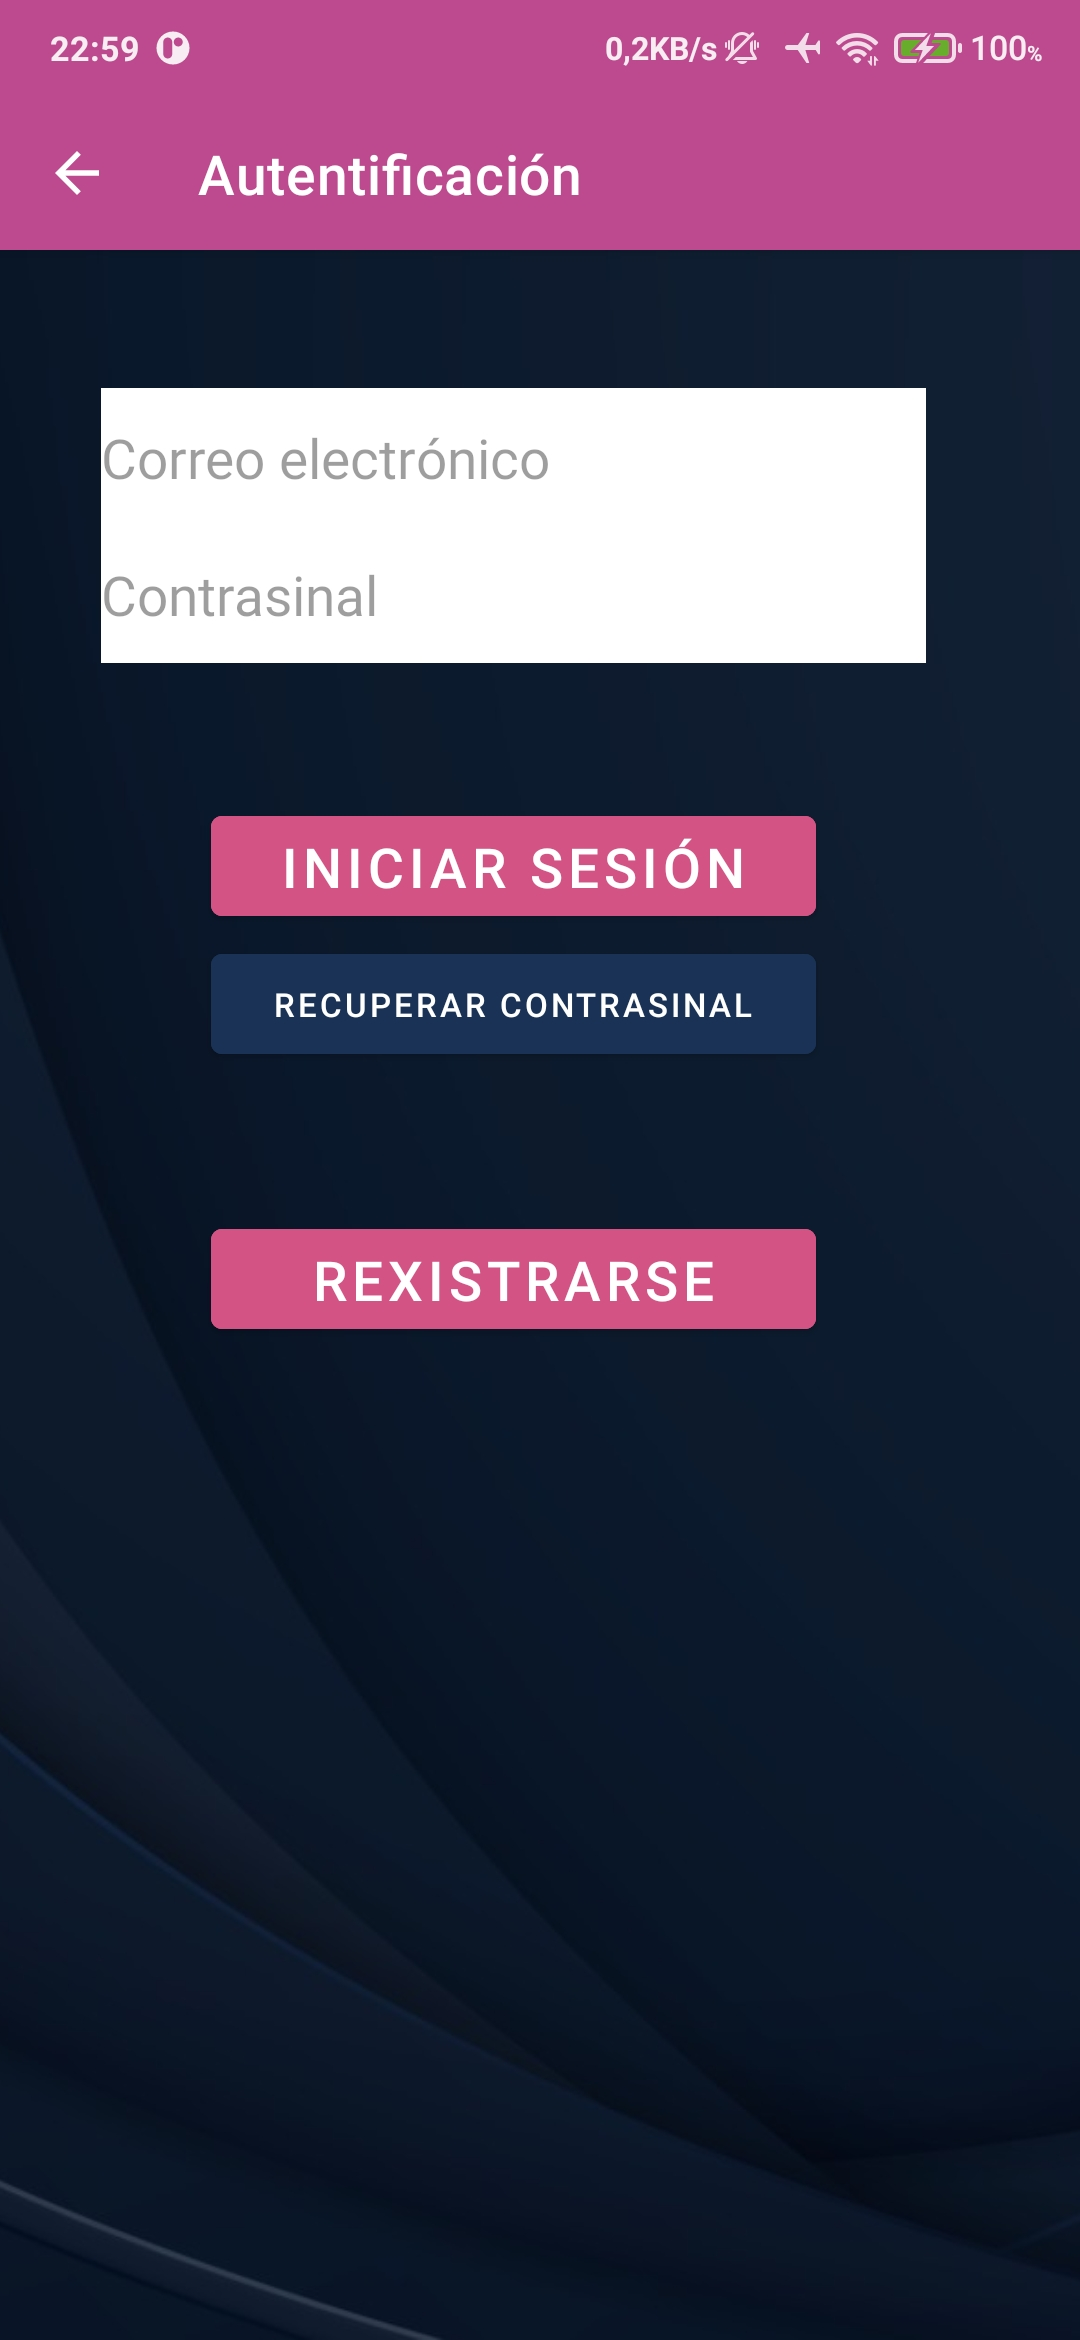
\includegraphics[scale=0.105]{imaxes/auth.jpg}\\[30 pt]
\end{center}
A prioridade de implementación das funcionalidades seguirá a orde descrita anteriormente, sendo o menú principal a primeira funcionalidade en ser implementada, o modo multixogador o último.\\
\section{Traballos futuros}
En traballos futuros pódense engadir novas funcionalidades como levar a conta de partidas gañadas e perdidas (pódense calcular estatísticas como porcentaxes de éxito ou número de intentos medios para obter unha victoria) en calquera dos dous modos, para isto faría falta outra base de datos a maiores, por último conviría desenvolver un multixogador en liña para máis de dous xogadores.\\
\\
Plantexamos elaborar tamén un proceso de testeo da aplicación coa axuda de usuarios e distintos tipos de probas de validación do software. Se se chegase a distribuír a aplicación cumpriría mantela con parches e actualizacións.

Tamén se considera a idea de seguir un modelo para o software da aplicación como pode ser o MVC que separa a vista do modelo mediante un controlador. Sería importante engadir soporte para diferentes idiomas e dispositivos en función da súa pantalla e do tamaño de fonte definido polo usuario a nivel de sistema operativo. De momento solo está pensado para estes parámetros en modo predeterminado.
 \let\cleardoublepage=\clearpage 